
 \begin{center}
 \textbf{
 %\dots
\og 
Ils ont témoigné de ce qu’ils ont vu
 \fg{}
 %\dots
 }
 \end{center}

\begin{wrapfigure}{l}{1.0cm}
\vspace{-0.5cm}
	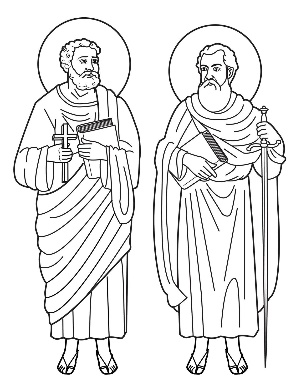
\includegraphics[scale=0.7]{../images/pierre_paul}
\end{wrapfigure}
Le mardi dernier, toute l’Église entière a célébré Saint Jean~Baptiste, le Saint Patron de notre Paroisse.
En ce dimanche nous célébrons les deux colonnes de l’Église Catholique Romaine. Tous les trois ont en commun d’avoir été témoins du Christ jusqu’au martyre. Jean~Baptiste, est celui-là, qui a proclamé dans le désert la venue du Messie. Quant à Pierre et Paul, ils ont annoncé la Bonne Nouvelle. Ils ont témoigné de l’œuvre de Dieu à travers leur ministère. Mais ils n’ont ni le même tempérament, ni la même ampleur dans le dessein. Les conditions dans lesquelles ils ont rencontré le Seigneur ont marqué différemment leur apostolat. En effet, différents dans leur action et dans leur caractère, mais ils ont été, tous deux choisis personnellement par le Christ. Ils se rejoignent dans la profondeur de leur foi et la ferveur de leur amour pour le Christ. Ils ont versé leur sang pour lui à Rome. En l’an 64 Saint Pierre et en l’an 67 pour Saint Paul. Ils demeurent pour l’Église deux grands hommes de foi, d’Esperance et de charité. Deux apôtres intrépides, infatigables et courageux. Si l’Église les réunit, les célèbre ensembles, c’est pour mieux mettre en lumière les merveilles de la grâce de Dieu dans le cœur vulnérable de deux amis et apôtres du Christ.

Parmi eux, c’est le bienheureux Pierre, qui est le premier.
Celui qui aimait fougueusement le Christ, et qui a eu le bonheur de s’entendre dire : \og Tu es Pierre et sur cette pierre je bâtirai mon Église \og{} (Mt 16,18).
Pour Paul tout a commencé sur la route de Damas, alors qu’il partait persécuter avec fierté les chrétiens, Jésus ressuscité vient à sa rencontre et l’aveugle de sa lumière. Après cela, il découvre alors en Jésus l’accomplissement du mystère du salut. Il consacre ainsi sa vie à parcourir la terre sans se soucier des difficultés et des persécutions pour annoncer Jésus-Christ.
\begin{wrapfigure}{l}{1.0cm}
\vspace{-0.5cm}
	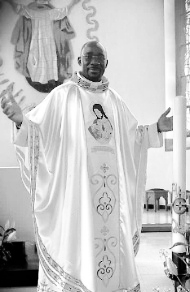
\includegraphics[scale=1.10]{../images/standing_daniel}
\end{wrapfigure}
Aujourd’hui, où nous les célébrons, nous pouvons dire sans ambages qu’ils ont répondu à la question fondamentale de la vie dont pose Jésus dans l’évangile de ce dimanche. : \og Pour vous qui suis-je ?\fg{}

Et nous quelle est notre réponse personnelle ?

Que le Seigneur nous donne la grâce de répondre à cette question en mettant nos pas dans ceux de Pierre et Paul, au cœur de notre vocation propre.

\begin{flushright}
Bonne méditation !
\textit{Père  Daniel  ETTÉ}
\end{flushright}


